\documentclass[border=0mm]{standalone}

\usepackage{import}
\subimport{../../../}{preamble.tex}

\usepackage{tikz}
\usetikzlibrary{calc}
\usepackage{pgfplots}
\usepgfplotslibrary{fillbetween}

\renewcommand{\t}{-5}

\begin{document}

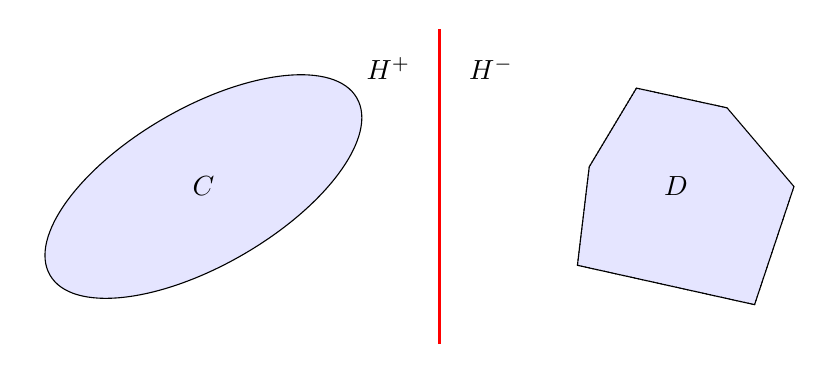
\begin{tikzpicture}[
  extended line/.style={shorten >=-#1},
  scale=0.5
  ]

  \begin{scope}[rotate=30]
    \coordinate (O) at (0,0);
    \coordinate (A) at (4.5,0);
    \coordinate (B) at (0,2);
    % draw ellipse
    \draw[black, fill=blue!10] (O) ellipse (4.5cm and 2.0cm);
    \node at (0,0) {$C$};
  \end{scope}

  \draw[line width=1pt, red] (6, -4) -- (6, 4);
  \node[left] at (5.5, 3) {$\red{H^+}$};
  \node[right] at (6.5, 3) {$\red{H^-}$};

  \begin{scope}[xshift=12cm, yshift=1cm]
    \node at (1.3, 1) (e1) {};
    \node at (-1, 1.5) (e2) {};
    \node at (3, -1) (e3) {};
    \node at (-2.2, -1/2) (e4) {};
    \node at (-2.5, -3) (e5) {};
    \node at (2, -4) (e6) {};

    \fill[blue!10] (e1.center) -- (e2.center)  -- (e4.center) -- (e5.center) -- (e6.center) -- (e3.center) -- cycle;
    \draw[black] (e1.center) -- (e2.center)  -- (e4.center) -- (e5.center) -- (e6.center) -- (e3.center) -- cycle;

    \draw[densely dotted]  (e1.center) -- (e2.center);
    \draw[densely dotted]  (e2.center) -- (e4.center);
    \draw[densely dotted]  (e4.center) -- (e5.center);
    \draw[densely dotted]  (e5.center) -- (e6.center);
    \draw[densely dotted]  (e6.center) -- (e3.center);
    
    \node at (0,-1) {$D$};
  \end{scope}

\end{tikzpicture}

\end{document}

%%% Local Variables:
%%% mode: latex
%%% TeX-master: t
%%% End:
